% watermarkデコードのアルゴリズム
Since DTMF modulation can be regarded as a special variety of frequency-shift keying (FSK), watermarks of AnnoTone embedded in media files can be extracted using common demodulation methods for FSK.
We implemented a decoder library using following algorithm, which could be used for creating applications utilizing annotations for content editing.

% 結果
\begin{figure}[htbp]
 \begin{center}
  \vspace{5mm}
  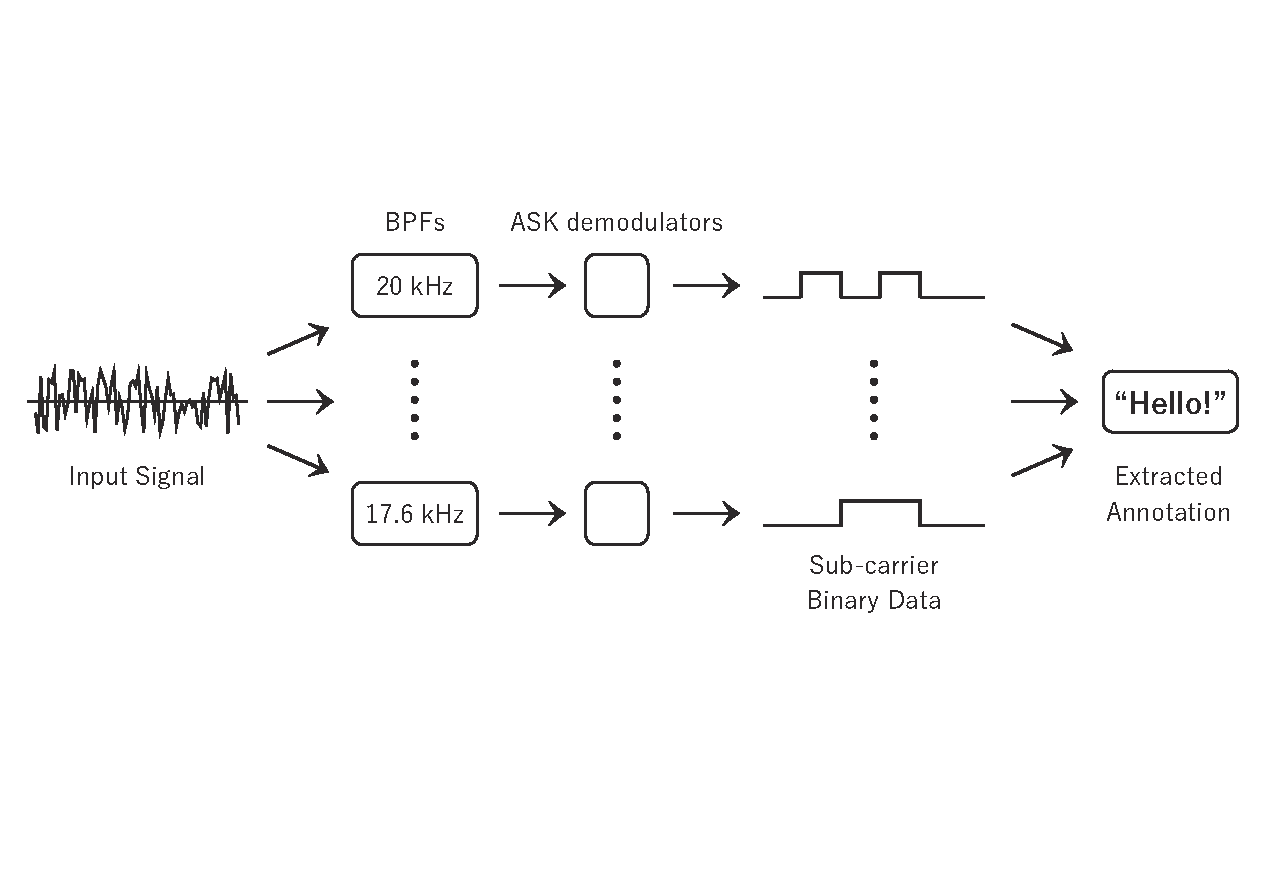
\includegraphics[width=130mm]{implementation_decode.pdf}
 \end{center}
 \caption{A schematic diagram of decoding algorithm.}
 \label{fig:impl_decd}
\end{figure}

% 形式を変換
Firstly, any kind of input file such as MPEG-2 format video is converted to pcm (.wav) file with 16 bit / 44.1 kHz sampling format using an external audio/video converter such as ffmpeg \cite{ffmpeg}.
% 各周波数ごとにBPF
Secondly, input signal is filtered by band-pass filters (BPFs) for each sub-carrier frequencies to extract each sub-carrier signals.
In our implementation, BPFs are designed as 199-tap finite impulse response filters.
After applying BPFs, binary states of each sub-carriers can be decided by a method for demodulating amplitude-shift keying (ASK).
% サンプル値の絶対値を取ってLPFに掛けてエンベロープを計算 
Thirdly, approximate envelopes of each sub-carrier signals are calculated by applying low-pass filter to them after taking absolute values of samples.
% エンベロープを簡単に2値化する
Fourthly, each envelope of frequency $f$ is binarized by a threshold $t(f)$ adaptively decided by the maximum value $max(f)$ and minimum value $min(f)$ of it as follows.

\begin{align}
t(f) = 0.9 \cdot min(f) + 0.1 \cdot max(f)
\end{align}

% タイムスタンプごとにDTMFデコードする
After this binarization, 4-bits values at each timestamp are scanned using the DTMF-encoding table mentioned above.
If the number of active sub-carriers is fewer than two, 4-bits value is regarded as invalid  at the timestamp, and if more than two sub-carriers are active, two sub-carriers with highest envelope values at the timestamp are used to decide the 4-bits value.

% 最後にパケット探索する
Finally, annotation packets are decoded from the scanned 4-bits value stream.
A start frame of a packet is identified by successive appearance of fixed value ``2'' for the half-length of a data frame.
After identifying a start frame, values for each data frames in the packet are decided by seeing 4-bits values at intervals of 10 ms.
% 続けて読み込むパケット長はlength frameから決定する
The number of data frames to read continuously is decided from the second data frame of the packet.
% 1パケット読み込み終わったらCRC-16チェックし、誤り検出されなかったら透かしとして確定する
After reading all data frames of a packet, it is extracted as an annotation if it passes CRC-8 error detection.